\section{Ejercicio 2: El Imperio contraataca}

    % Describir detalladamente el problema a resolver dando ejemplos del mismo y sus soluciones.
    \subsection{Descripción del problema}

    \begin{figure}[ht]
        \begin{center}
            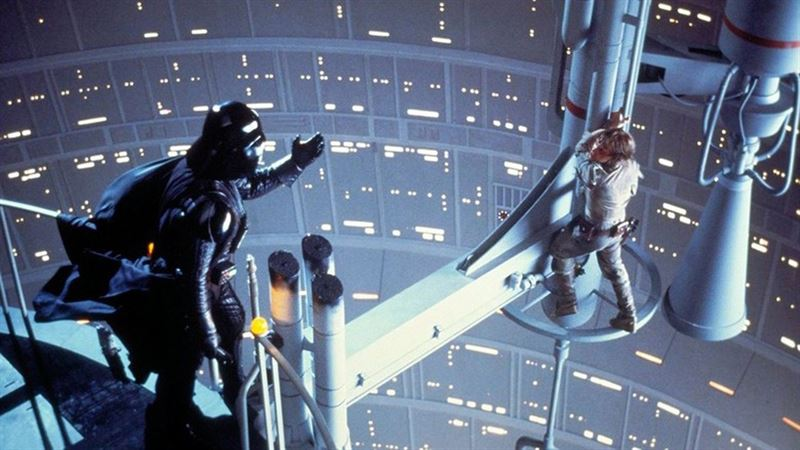
\includegraphics[width=10cm]{imagenes/el_imperio_contraataca.jpg}
            \caption*{``¡Prestame atención a mí, soy tu padre!''}
        \end{center}
    \end{figure}

    Luke debe informarle a todos sus aliados para que estén al tanto del contraataque del Imperio. Parte del planeta Hoth, conocido como planeta 0, y quiere que la noticia llegue a todos los planetas.

    En cada planeta hay infinitos halcones milenarios. Los halcones milenarios consumen una determinada de combustible cada un millón de kilómetros.

    Una vez que un halcón milenario llega a un planeta, de éste pueden salir cualquier cantidad de halcones para seguir advirtiendo a los rebeldes de otros planetas.

    Los halcones milenarios no pueden viajar por cualquier lado, solo por determinadas rutas espaciales. Cada ruta conecta exactamente dos planetas, y recorrer cada ruta consume una determinada cantidad de combustible. Además, se sabe que existe al menos una forma de llegar desde cualquier planeta a cualquier otro a través de rutas espaciales.

    Se pide encontrar cuál es la mínima cantidad de combustible necesaria para entregar el mensaje en todos los planetas. Además, se debe indicar de qué planeta proviene la nave que entrega el mensaje, para cada planeta excepto el 0.

    Se pide que el algoritmo tenga una complejidad temporal $\ord(M$ log $M)$.

    \vspace{1.25em}

    \textbf{Formato de entrada}: La primera línea consta de un entero positivo \texttt{N}, que indica la cantidad de planetas, y un entero positivo M, que indica la cantidad de rutas espaciales. A continuación de esta línea siguen \texttt{M} líneas con enteros \texttt{Ai}, \texttt{Bi} y \texttt{Li}, siendo \texttt{Ai} y \texttt{Bi} los extremos de la ruta y \texttt{Li} la cantidad de litros que se gastan al recorrer esa ruta ($0 \leq \mathtt{Ai} \neq \mathtt{Bi} \leq N-1$). La entrada contará con el siguiente formato:

    \begin{verbatim}
    N M
    A0 B0 L0
    A1 B1 L1
    ...
    AM-1 BM-1 LM-1\end{verbatim}

    \vspace{.8em}

    \textbf{Formato de salida}: La primera línea debe contener la cantidad mínima de litros \texttt{L} necesarios para informar a toda la alianza sobre esta noticia, seguida de $N-1$ líneas que indican desde qué planeta se viaja para informar de la situación a cada planeta (el vecino inmediato desde el cual se viaja). El formato debe ser el siguiente:

    \begin{verbatim}
    L
    I1
    I2
    ...
    IN-1\end{verbatim}

    indicando que al planeta \texttt{i} se le informa de la situación con una nave que parte del planeta \texttt{Ii}.

    \vspace{.8em}

    A continuación se incluyen, a modo de ejemplo, una posible entrada y una
    salida correcta para la misma:

    \vspace{.5em}
    \begin{tabular}{l @{\hskip 4em} l}
    \textbf{Entrada} & \textbf{Salida} \\
    \texttt{4 4}     & \texttt{4}      \\
    \texttt{0 1 1}   & \texttt{0}      \\
    \texttt{1 2 2}   & \texttt{1}      \\
    \texttt{1 3 5}   & \texttt{2}      \\
    \texttt{2 3 1}   &                 \\
    \end{tabular}
    \vspace{.5em}

    \begin{figure}[H]
        \centering
        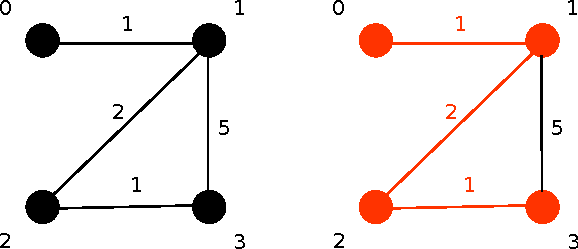
\includegraphics{imagenes/ej2_modelo_1.pdf}
        \caption*{Ejemplo de entrada}
        \label{ej2:ejemplo}
    \end{figure}

    Es importante observar que puede haber más de una salida distinta válida.

    % Explicar de forma clara, sencilla, estructurada y concisa, las ideas
    % desarrolladas para la resolución del problema. Utilizar pseudocódigo y
    % lenguaje coloquial (no código fuente). Justificar por qué el
    % procedimiento resuelve efectivamente el problema.
    \subsection{Solución propuesta}

    \subsubsection{Modelo}

    El hecho de que los planetas se encontraran unidos mediante rutas, y que
    cada una de ellas conectara exactamente dos planetas, permitió encarar la
    resolución del problema modelando el sistema planetario mediante un
    grafo, donde cada planeta es un vértice y cada ruta es un eje.

    Para representar los distintos costos de utilizar una u otra ruta
    espacial, se consideró un grafo ponderado, utilizando como peso de cada
    eje la cantidad de combustible que cuesta recorrer la ruta
    correspondiente. Por otra parte, el hecho de que siempre exista forma de
    viajar entre dos planetas equivale a decir que el grafo es conexo.

    Sea $G$ el grafo cuyo conjunto de vértices son los planetas y su conjunto
    de aristas, las rutas espaciales. Notar que $G$ es un grafo conexo y
    sus aristas tienen pesos no negativos. Bajo este modelo, el problema que
    busca resolverse se traduce en hallar un subgrafo $T$ de $G$, de forma tal
    que:
    \begin{enumerate}
        \item Todos los nodos de $G$ sean nodos de $T$.
        \item Para algún nodo $v_0 \in V(G)$ (representando al planeta Hoth),
        exista en $T$ un camino entre $v_0$ y cualquier otro nodo. Dado que
        $T$ es un grafo no dirigido, esto equivale a pedir que $T$ sea conexo.
        \item La suma de los pesos de todos los ejes $T$ sea mínima con
        respecto a todos los subgrafos de $G$ que cumplen los dos puntos
        anteriores.
    \end{enumerate}

    \begin{lema}
    Sea $G$ un grafo con pesos no negativos, y $T \subseteq G$ un árbol
    generador mínimo de $G$. Entonces $T$ cumple las tres propiedades recién
    enunciadas.
    \end{lema}
    \begin{proof}
    Sabemos que $T$ cumple los dos primeros ítems, por definición de árbol
    generador mínimo.
    Supongamos ahora que no se cumple el tercer punto, es decir, que existe
    otro subgrafo de $G$, $H$, que también cumple las primeras dos propiedades
    y tal que el peso total de sus aristas es estrictamente menor que el de
    $T$.

    Por el segundo punto, sabemos que $H$ es conexo, por lo que tiene al menos
    un \acr{agm} $\tilde{H}$ que también cumple las primeras dos
    propiedades enunciadas. Por el primer punto, $H$ contiene todos los
    nodos de $G$, así que $\tilde{H}$ también es árbol generador de $G$.
    Dado que las aristas de $H$ tienen pesos no negativos, y todas las aristas
    de $\tilde{H}$ están en $H$, el peso total de las aristas de $\tilde{H}$
    es menor o igual que la de $H$ y, por transitividad, también que el de
    $T$. Es decir, $H$ es un árbol generador de $G$ cuyo peso total es menor
    que el de $T$, lo cual cual contradice el hecho de que que $T$ es un \acr
    {agm} de $G$.

    Esto prueba que no puede existir tal subgrafo $H$, es decir, que $T$
    cumple también con la tercer propiedad.
    \end{proof}

    Del lema anterior, se sigue directamente que, para resolver el problema
    planteado, resulta correcto modelarlo mediante un grafo de la manera
    descripta y, a continuación, buscar un árbol generador mínimo de dicho
    grafo.

    \subsubsection{Implementación}
    Para resolver el problema de buscar un \acr{agm} de un grafo,
    se realizó una implementación del algoritmo de Prim, cuyo pseudocódigo
    se incluye como Algoritmo \ref{algo:prim}.

    \begin{algorithm}
        \caption{Algoritmo de Prim}
        \label{algo:prim}

        \Input{Un grafo $G$ de $N$ nodos y $M$ aristas, dado por un vector de
        listas de adyacencia}
        \Output{Un árbol generador mínmo de $G$, dado como un vector
        conteniendo el predecesor de cada nodo, y el peso total de dicho árbol}
        $predecesores$ $\gets$ vector de longitud $N$ \;
        $peso\ total$ $\gets$ $0$ \;
        $vertices$ $\gets$ cola de prioridad vacía \;
        encolar $v_0$ en $vertices$ con prioridad $0$ \;
        \ForEach{$i$ entre $1$ y $N-1$} {
            encolar $v_i$ en $vertices$ con prioridad $\infty$ \;
        }
        \While{$vertices$ no esté vacía} {
            $v$ $\gets$ $vertices$.desencolar() \;
            marcar $v$ como visitado \;
            $peso\ total$ $\gets$ $peso\ total$ + prioridad de $v$ en $vertices$ \;
            \ForEach{vecino $u$ de $v$}{
                \If{$u$ no está marcado como visitado} {
                    $p$ $\gets$ peso de la arista $(v,u)$ en $G$ \;
                    \If{$p < $ prioridad de $u$ en $vertices$} {
                        actualizar prioridad de $u$ en $vertices$ a $p$ \;
                        $predecesores$[$u$] $\gets$ $v$ \;
                    }
                }
            }
        }
        \Return{$predecesores$, $peso\ total$}
    \end{algorithm}

    El algoritmo de Prim empieza agregando al árbol un nodo cualquiera del
    grafo. Luego, comienza a construir la solución, incorporando el eje de
    menor peso que sea adyacente a dicho nodo, y sumando así al árbol su otro
    extremo. Este proceso se repite, añadiendo en cada iteración la arista de
    menor peso que tenga por extremos un nodo dentro y otro fuera del árbol,
    hasta que ya no queden nodos para agregar al árbol.

    Existen diversas implementaciones de este algoritmo, que varían
    principalmente en las estructuras de datos utilizadas durante el proceso,
    y que presentan distintos niveles de eficiencia en términos temporales y
    espaciales. En este caso, se optó por una solución derivada de la
    típica implementación del algoritmo de caminos mínimos de Dijkstra,
    utilizando una cola de prioridad sobre un \emph{heap} binario.

    En una iteración determinada, esta cola contiene todos los nodos del grafo
    sobre los que aún no se ha iterado. Antes de la primera iteración, todos
    los nodos son agregados a la cola con prioridad $\infty$, excepto el nodo
    $v_0$, al que se le asigna una prioridad $0$. Esto último es una pequeña
    modificación al algoritmo original, cuyo objetivo es asegurarse de
    que $v_0$ sea el primer nodo en ser desencolado, ya que se desea obtener
    un \acr{agm} enraizado en este vértice en particular.

    Como cada nodo comienza teniendo una prioridad de $\infty$, que recién
    es modificada cuando se suma al árbol uno de sus nodos adyacentes,
    resulta claro que en una iteración determinada, un nodo que se encuentra
    encolado tiene una prioridad menor que $\infty$ si y solo si es adyacente
    a algún otro que ya forma parte del árbol. Más aún, su prioridad
    corresponde al mínimo entre los pesos de todas las aristas que comparte
    con algún nodo del árbol. El ciclo principal del algoritmo se encarga de
    mantener este invariante: cada vez que un nodo se agrega al árbol, se
    recorren sus vecinos, y si el eje que lo une a alguno de ellos tiene un
    valor menor que la prioridad del mismo, esta prioridad es actualizada.

    Teniendo en cuenta lo anterior, es inmmediato que al final de cada
    iteración, la arista de mínimo peso con un extremo dentro y el otro fuera
    del árbol tiene, como este último extremo, al nodo cuya prioridad en la
    cola es la de mínimo valor numérico. Esta es la razón de que, al comienzo
    de la siguiente iteración, este será el nodo seleccionado para agregar al
    árbol, implementando de esta forma el procedimiento propuesto por el
    algoritmo de Prim.

    El problema requiere, además de una descripción del árbol dada por el
    predecesor de cada uno de los nodos, que se compute el peso total de sus
    aristas. Para lograr esto se aprovecha que, cuando un nodo es marcado como
    visitado, su predecesor ya no será modificado, por lo que se sabe que
    la arista que lo une a su padre formará parte del árbol final. Así, el
    peso total del árbol se va calculando en forma incremental: cada
    vez que se marca un nodo como visitado, se suma al peso total el peso de
    la arista entre él y su predecesor.

    \subsubsection{Detalles implementativos}
    Todas las rutinas arriba descriptas fueron implementadas en lenguaje C++.
    Se hizo uso de la clase \texttt{vector}, provista en la biblioteca
    estándar del lenguaje, en forma directa y también como contenedor
    subyacente a la cola de prioridad. Esta última debió ser implementada en
    forma propia para poder cubrir los requisitos de complejidad del problema.

    A continuación se describe la forma en que fue implementada esta cola de
    prioridad. La estructura básica es un clásico
    \emph{min-heap} binario, almacenado en un vector. Cada posición de este
    vector contiene una tupla de dos valores enteros: la prioridad del
    elemento y el valor del mismo. Se implementan internamente las
    operaciones típicas de \emph{subir} y \emph{bajar} un elemento, que
    permiten mantener el invariante de \emph{heap}. De esta forma puede
    obtenerse el elemento con prioridad mínima en tiempo $\Theta(1)$,
    mientras que desencolar este elemento tiene complejidad $\ord(\log(N))$.
    También puede decidirse en $\Theta(1)$ si la cola está vacía.

    La principal diferencia con la típica implementación de \emph{heap} es
    que permite modificar la prioridad de un elemento en tiempo
    logarítmico. Sin estructuras auxiliares, esto tendría un costo lineal, ya
    que debe buscarse al elemento deseado antes de poder modificarlo. Una vez
    encontrado, reacomodar el \emph{heap} con la nueva prioridad tiene
    complejidad logarítmica.

    La solución fue incorporar una estructura adicional para poder encontrar
    un elemento dado de forma eficiente. Se barajaron varias opciones, pero
    finalmente se decidió aprovechar el hecho de que los elementos de la cola
    serían números naturales en un rango acotado entre $0$ y algún valor $k$
    (los índices de los nodos del grafo a procesar). Se incorporó entonces un
    vector de tamaño $k$ que almacena, en la posición $i$-ésima, la posición
    del elemento $i$ en el vector que representa al heap. De esta forma no
    solo puede actualizarse la prioridad de un elemento de forma eficiente
    ($\ord(\log(N))$) sino también consultar la prioridad de cualquier
    elemento en tiempo constante.

    Para simplificar la implementación, se decidió omitir la operación de
    agregar un elemento a la cola. Se incorporó, en cambio, un constructor que
    toma un parámetro $k$ e inicializa una cola que contiene a todos los
    naturales entre $0$ y $k-1$ inclusive, todos con prioridad $\infty$,
    donde una prioridad infinita se indica mediante el tope de representación
    del tipo \texttt{int} en C++. El costo de esta inicialización es lineal
    en el valor de $k$. Esta funcionalidad resulta suficiente para
    el uso particular que se le da a la estructura en este trabajo.

    Es importante señalar que, debido a estas particularidades de la
    estructura utilizada, el primer ciclo del pseudocódigo del Algoritmo
    \ref{algo:prim} no resulta necesario, ya que queda reemplazado en la
    práctica por la inicialización de la cola de prioridad. Asimismo, la
    operación de encolar al elemento $v_0$ con prioridad $0$ es sustituida
    por actualizar su prioridad, ya que el elemento está presente en la cola
    desde su inicialización.

    % Deducir una cota de complejidad temporal del algoritmo propuesto (en
    % función de los parámetros que se consideren correctos) y justificar por
    % qué el algoritmo la cumple. Utilizar el modelo uniforme.
    \subsection{Complejidad teórica}
    Para elaborar una cota teórica para la complejidad del algoritmo
    presentado, se considerará que el grafo a procesar tiene $N$ nodos y $M$
    aristas.
    Teniendo en cuenta, además, que el grafo es conexo, puede asumirse que
    $M \geq N-1$, lo cual implica que $N \in \ord(M)$.

    No se detallará en los cálculos el tiempo necesario para la lectura de
    los datos, la creación de las listas de adyacencia a partir de las listas
    de aristas brindadas como entrada y la escritura de la salida. No
    obstante, estas operaciones tienen en todos los casos un costo no
    superior a $\ord(M)$.

    \vspace{1.25em}

    La implementación del algoritmo de Prim comienza inicializando una cola
    de prioridad de tamaño $N$, de la forma descripta en la sección anterior,
    con un costo de $\Theta(N)$. Inmediatamente después se modifica la
    prioridad de un elemento, con una complejidad de $\ord(\log(N))$.

    A continuación se ejecuta el ciclo principal del algoritmo. En cada
    iteración de este ciclo se remueve un elemento de la cola recién
    mencionada, terminando cuando la cola se vacía; es decir, el ciclo se
    ejecuta exactamente $N$ veces.

    Cada iteración del ciclo se corresponde con un nodo del grafo. Dentro de
    la misma, en primer lugar, se desencola el nodo de la cola de prioridad,
    lo cual tiene un costo de $\ord(\log(N))$. Luego se realizan dos
    operaciones de costo constante ($\Theta(1)$): se marca el nodo como
    visitado y se suma su peso al peso total. A continuación se ejecuta a su
    vez otro ciclo que itera sobre los vecinos del nodo, es decir, se repite
    $\operatorname{deg}(v_i)$ veces. En el caso de que el vértice no
    pertenezca al árbol parcial generado hasta el momento, se obtiene
    el peso de la arista correspondiente y se verifica si es menor
    que la prioridad actual del nodo en la cola; todas estas operaciones
    pueden realizarse en tiempo constante. En caso afirmativo la prioridad
    debe ser actualizada, lo cual tiene un costo de $\ord(\log(N))$. Esto
    implica que la iteración $i$-ésima del ciclo principal tiene una
    complejidad de peor caso de
    $\ord \left(\log(N) + \operatorname{deg}(v_i) \times \log(N) \right)$.

    Sumando esta complejidad para todas las iteraciones del ciclo, obtenemos
    una complejidad total de
    \[ \begin{aligned}
    \sum_{i=0}^{N} \ord \left( \log(N) + \operatorname{deg}(v_i)
        \times \log(N) \right)
            &= \ord \left( \sum_{i=0}^{N} (1+\operatorname{deg}(v_i))
                \times \log(N) \right) \\
            &= \ord \left( \left( N + \sum_{i=0}^{N}
                \operatorname{deg}(v_i) \right) \times \log(N) \right) \\
            &= \ord \left( (N + M) \times \log(N) \right) \\
            &= \ord \left( M \times \log(N) \right)
    \end{aligned} \]

    Esta complejidad no se ve afectada por las operaciones de inicialización
    antes descriptas, puede deducirse una cota teórica para
    la complejidad temporal de la solución presentada de:
    \[ \ord(N + \log(N) + M \times \log(N)) = \ord(M \times \log(N)) \]

    % Realizar experimentación para medir la performance, usando un conjunto
    % de casos de test que permitan observar los tiempos de ejecución en
    % función de los parámetros de entrada, tanto para instancias aleatorias
    % (detallando cómo fueron generadas) como para instancias particulares
    % (peor/mejor caso, por ejemplo). Presentar en forma gráfica una
    % comparación entre los tiempos medidos y la complejidad teórica y extraer
    % conclusiones.
    \subsection{Experimentación}

    Se realizaron pruebas experimentales para verificar que el tiempo de ejecución del algoritmo cumpliera con la cota asintótica de $\ord(M \times log(N))$, demostrada teóricamente. Se realizaron las siguientes pruebas:

    \begin{itemize}
    \item Pruebas con instancias en donde se mantiene la cantidad de nodos fija y se hacen variar las aristas.
    \item Pruebas con instancias en donde se mantiene la cantidad de aristas fija y se hacen variar los nodos.
    \item Pruebas con instancias en donde se varía la cantidad de aristas $M$ y de nodos $N$, siempre cumpliendo que $M = N  - 1$, es decir, que cada grafo construido es un árbol.
    \item Pruebas con instancias en donde se varía la cantidad de aristas $M$ y de nodos $N$, siempre cumpliendo que $M = \frac{N \times (N - 1)}{2}$.
    \end{itemize}

    Se generaron 40 instancias de prueba en cada uno de estos escenarios. En cada caso, se ejecutaron 30 repeticiones del algoritmo, midiendo cada vez el tiempo de ejecución y tomando luego el promedio entre los resultados obtenidos.

    Debido a los picos en el tiempo de ejecución en las primeras corridas del programa, tendiendo los valores a estabilizarse con las sucesivas corridas, se decidió, para minimizar la varianza de los datos obtenidos, tratar a las primeras 10 repeticiones de cada instancia como \textit{outliers}, y promediar solo los valores de las últimas 20.

    Todas las instancias utilizadas para estas pruebas se generaron de manera aleatoria.

    A continuación se detalla la notación utilizada en los gráficos para referirse a los mismos.

    \begin{itemize}
        \item $A$: Árbol generado de manera aleatoria. Para cada valor de $M$, se genera un grafo de $N = M+1$ nodos. A continuación, se van agregando aristas al grafo de forma aleatoria, asegurándose de que no se formen ciclos, hasta completar $M$ aristas.
        \item $G$: Grafo conexo generado de manera aleatoria. Se genera un árbol de forma aleatoria al cual se le agregan aristas, también al azar, hasta completar las $M$ aristas.
        \item $K$: Grafo completo. Para cada valor de $M$ se considera un grafo completo con $\frac{1 + \sqrt{1 + 8 \times M}}{2}$ nodos.
    \end{itemize}

    \renewcommand\constante{10}

    En la Figura \ref{fig:exp2:n_fijo} se reflejan los resultados de mantener una cantidad $N$ de nodos fija, variando la cantidad de aristas $M$ de los grafos. El valor en el que se fijó $N$ fue de 400. Los valores de $M$ se encuentran entre 399 y 79800. Estos valores corresponden a la mínima y máxima cantidad de aristas que un grafo conexo con $N$ fijo puede tener, respectivamente. Notar que necesitamos que el grafo sea conexo para cumplir con los requisitos del enunciado del problema. La mínima cantidad de aristas de un grafo conexo de $N$ nodos es de $M = N - 1$, y la máxima es el grafo completo, $M = \frac{N(N - 1)}{2}$.

    La complejidad del algoritmo es de orden $\ord(M \times log(N))$, pero como en esta prueba $N$ es constante, la complejidad temporal debería ser lineal en la cantidad de aristas. Es por eso que se ilustra la cota teórica de $c \times M$ (el valor de $c$ utilizado es \constante).

    \begin{figure}[H]
        \centering
        \caption{}
        \label{fig:exp2:n_fijo}
        \begin{tikzpicture}
            \begin{axis}[
                    title={Cantidad de nodos fija $N = 1000$},
                    xlabel={Cantidad de aristas($M$)},
                    ylabel={Tiempo de ejecución (nanosegundos)},
                    scaled x ticks=false,
                    scaled y ticks=false,
                    enlargelimits=0.05,
                    width=0.5\textwidth,
                    height=0.5\textwidth,
                    legend pos=south east,
                    legend cell align=left,
                    xmin=1
                ]
                \addplot[color=black] table[x index=0,y index=1]{../exp/elImperioContraatacaNFijo};
                \addplot[color=red] table[x index=0, y expr={x*\constante}]{../exp/elImperioContraatacaNFijo};
                \legend{$G$ (Grafo conexo), $c \times M$ ($c = \constante$)}
            \end{axis}
        \end{tikzpicture}
    \end{figure}

    \renewcommand\constante{24000000}

    En la Figura \ref{fig:exp2:m_fijo} se reflejan los resultados de mantener una cantidad $M$ de aristas fija, variando la cantidad de nodos $N$ de los grafos. El valor en el que se fijó $M$ fue de 400000. Los valores de $N$ se encuentran entre 895 y 400001. Estos valores corresponden a la mínima y máxima cantidad de nodos que un grafo conexo con $M$ fijo puede tener, respectivamente. La mínima cantidad de nodos de un grafo conexo de $M$ aristas es el grafo completo, $N = \frac{1 + \sqrt{1 + 8M}}{2}$, y la máxima es de $N = M + 1$.

    Así como en el experimento anterior, la complejidad temporal del experimento varía de la del algoritmo, ya que $M$ se mantiene constante. Esta debería ser logarítmica en la cantidad de nodos. Es por eso que se ilustra la cota teórica de $c \times log(N)$ (el valor de $c$ utilizado es \constante).

    \begin{figure}[H]
        \centering
        \caption{}
        \label{fig:exp2:m_fijo}
        \begin{tikzpicture}
            \begin{axis}[
                    title={Cantidad de nodos fija $M = 400000$},
                    xlabel={Cantidad de nodos($N$)},
                    ylabel={Tiempo de ejecución (nanosegundos)},
                    scaled x ticks=false,
                    scaled y ticks=false,
                    enlargelimits=0.05,
                    width=0.5\textwidth,
                    height=0.5\textwidth,
                    legend pos=south east,
                    legend cell align=left,
                    xmin=1
                ]
                \addplot[color=black] table[x index=0,y index=1]{../exp/elImperioContraatacaMFijo};
                \addplot[color=red] table[x index=0, y expr={ln(x)*\constante}]{../exp/elImperioContraatacaMFijo};
                \legend{$G$ (Grafo conexo), $c \times log(N)$ ($c = \constante$)}
            \end{axis}
        \end{tikzpicture}
    \end{figure}

    \renewcommand\constante{5}

    En la Figura \ref{fig:exp2:arboles} se reflejan los resultados de variar la cantidad de aristas y de nodos, donde cada grafo en este experimento es un árbol. Estos resultados se contrastan con la ilustración de la cota teórica de complejidad del algoritmo, $c \times M \times log(N)$ (el valor de $c$ utilizado es \constante).

    \begin{figure}[H]
        \centering
        \caption{}
        \label{fig:exp2:arboles}
        \begin{tikzpicture}
            \begin{axis}[
                    title={Árboles},
                    xlabel={Cantidad de aristas($M$)},
                    ylabel={Tiempo de ejecución (nanosegundos)},
                    scaled x ticks=false,
                    scaled y ticks=false,
                    enlargelimits=0.05,
                    width=0.5\textwidth,
                    height=0.5\textwidth,
                    legend pos=south east,
                    legend cell align=left,
                    xmin=1
                ]
                \addplot[color=black] table[x index=0,y index=1]{../exp/elImperioContraatacaArboles};
                \addplot[color=red] table[x index=0, y expr={x*ln(x + 1)*\constante}]{../exp/elImperioContraatacaArboles};
                \legend{$A$ (Árbol), $c \times M \times log(N)$ ($c = \constante$)}
            \end{axis}
        \end{tikzpicture}
    \end{figure}

    En la Figura \ref{fig:exp2:arboles:cociente} se muestra el cociente entre los resultados obtenidos de la experimentación con árboles y la función $M \times log(N)$.

    Se debe observar que es posible utilizar $N$ para el cociente debido a que los experimentos se realizan con árboles, por lo que variar $M$ repercute en $N$ siempre de la misma forma, $N = M + 1$. Se puede ver que el cociente se mantiene constante.

    \begin{figure}[H]
        \centering
        \caption{}
        \label{fig:exp2:arboles:cociente}
        \begin{tikzpicture}
            \begin{axis}[
                    title={},
                    xlabel={Cantidad de aristas($M$)},
                    ylabel={nanosegundos $/$ $(M \times log(N))$},
                    scaled x ticks=false,
                    scaled y ticks=false,
                    enlargelimits=0.05,
                    width=0.5\textwidth,
                    height=0.5\textwidth,
                    legend pos=south east,
                    legend cell align=left,
                    xmin=1,
                    ymin=0,
                    ymax=10
                ]
                \addplot[color=black] table[x index=0,y expr={\thisrowno{1} / (x * ln(x + 1))}]{../exp/elImperioContraatacaArboles};
                \addplot[color=red] table[x index=0, y expr={\constante}]{../exp/elImperioContraatacaArboles};
                \legend{$\frac{A}{M \times log(N)}$, $c = \constante$}
            \end{axis}
        \end{tikzpicture}
    \end{figure}

    \renewcommand\constante{0.8}

    A continuación se exponen los resultados obtenidos del experimento con grafos completos. En la Figura \ref{fig:exp2:completos} pueden verse reflejados. Para este experimento se varía la cantidad de aristas $M$ y de nodos $N$ cumpliendo que $M = \frac{N \times (N - 1)}{2}$. Estos resultados se contrastan con la ilustración de la cota teórica de complejidad del algoritmo, $c \times M \times log(N)$ (el valor de $c$ utilizado es \constante).

    \begin{figure}[H]
        \centering
        \caption{}
        \label{fig:exp2:completos}
        \begin{tikzpicture}
            \begin{axis}[
                    title={Completos},
                    xlabel={Cantidad de nodos($N$)},
                    ylabel={Tiempo de ejecución (nanosegundos)},
                    scaled x ticks=false,
                    scaled y ticks=false,
                    enlargelimits=0.05,
                    width=0.5\textwidth,
                    height=0.5\textwidth,
                    legend pos=south east,
                    legend cell align=left,
                    xmin=1
                ]
                \addplot[color=black] table[x index=0,y index=1]{../exp/elImperioContraatacaCompletos};
                \addplot[color=red] table[x index=0, y expr={(x - 1)*x/2*ln(x)*\constante}]{../exp/elImperioContraatacaCompletos};
                \legend{$K$ (Grafo completo), $c \times M \times log(N)$ ($c = \constante$)}
            \end{axis}
        \end{tikzpicture}
    \end{figure}

    En la Figura \ref{fig:exp2:completos:cociente} se muestra el cociente entre los resultados obtenidos de la experimentación con grafos completos y las funciones $M$ y $M \times log(N)$ respectivamente.

    Se debe observar que es posible utilizar $N$ para el cociente debido a que los experimentos se realizan con grafos completos, por lo que variar $N$ repercute en $M$ siempre de la misma forma, $M = \frac{N \times (N - 1)}{2}$. Se puede ver que el cociente no superará a la constante.

    \begin{figure}[H]
        \centering
        \caption{}
        \label{fig:exp2:completos:cociente}
        \begin{tikzpicture}
            \begin{axis}[
                    title={},
                    xlabel={Cantidad de nodos($N$)},
                    ylabel={nanosegundos $/$ $(M \times log(N))$},
                    scaled x ticks=false,
                    scaled y ticks=false,
                    enlargelimits=0.05,
                    width=0.5\textwidth,
                    height=0.5\textwidth,
                    legend pos=south east,
                    legend cell align=left,
                    xmin=1,
                    ymin=0
                ]
                \addplot[color=black] table[x index=0,y expr={\thisrowno{1} / ((x - 1) * x * ln(x))}]{../exp/elImperioContraatacaCompletos};
                \addplot[color=red] table[x index=0, y expr={\constante}]{../exp/elImperioContraatacaCompletos};
                \legend{$\frac{K}{M \times log(N)}$, $c = \constante$}
            \end{axis}
        \end{tikzpicture}
    \end{figure}

    El análisis expuesto de los datos recopilados presenta evidencia empírica sobre la pertinencia de la cota de complejidad demostrada teóricamente.
